\chapter[Referencial Teórico]{Referencial Teórico}

\section{Linguagens Formais}
\label{sec:languages}


Dentro do inglês letras, palavras e sentenças são entidades distintas.
Também é verdade que existem agrupamentos, isto é, conjuntos de letras
formam palavras e conjuntos de palavras formam sentenças. Contudo, 
nem todos esses conjuntos são válidos \cite{cohen1986}.

Esse tipo de relação também é válido para linguagens em computadores.
Por exemplo, na linguagem de programação \textit{C}, conjuntos de caracteres formam comandos
e um conjunto desses comandos formam programas e estes também podem ser válidos ou não \cite{cohen1986}.

O estudo de linguagens formais busca entender como funcionam as linguagens de maneira unificada 
e utilizando regras claras. Isto implica em definir sem ambiguidades, o que é uma linguagem e
como validar uma linguagem. O formalismo também pressupõe que esta área não busca
compreender a comunicação ou a interpretação subjetiva de textos \cite{cohen1986}.

Segundo \citeonline{cohen1986}, para definir uma linguagem de maneira formal 
existe um conjunto finito de unidades fundamentais chamdo alfabeto. Essas unidades
são chamadas de símbolos.

Uma sequência de símbolos é chamado \textit{string} e um conjunto específico dessas \textit{strings} 
que utiliza símbolos do alfabeto forma uma linguagem. Também seria possível existir uma \textit{string} vazia. 

Já segundo \citeonline{aho2006}, uma linguagem é qualquer conjunto de \textit{strings} contável
que usa símbolos de um alfabeto especificado.

Também segundo \citeonline{aho2006}, é possível fazer algumas operações com estas linguagens.
Por exemplo, dado duas linguagens em que L representa o conjunto de letras do inglês 
e D o conjunto de dígitos, podemos definir as operações da seguinte maneira:

\begin{itemize} 
    \item União ente linguagens é similar a operação em conjuntos, isto é a união de L e D significa
    todas as letras do alfabeto da linguagem L mais os dígitos do alfabeto da linguagem D.
    \item Concatenação de linguagens significa uma operação onde todas as cadeias de caracteres são
    formadas pegando todas as \textit{strings} da primeira linguagem e todas as \textit{strings} 
    da segunda linguagem em todas as combinações possíveis, por exemplo a concatenação de L com D
    significa uma outra linguagem que consiste do conjunto de \textit{strings} de dois símbolos, o primeiro
    da linguagem L e o subsequente da linguagem D.
    \item A operação \textit{kleene closure} de uma linguagem é o conjunto de \textit{strings} criadas concatenando a linguagem zero 
    ou mais vezes, por exemplo aplicar esta operação na linguagem L significa que palavras com zero ou mais letras
    são válidas na nova linguagem.
    \item A operação \textit{postive closure} de uma linguagem é o conjunto de \textit{strings} criadas concatenando a linguagem uma 
    ou mais vezes, ao aplicar esta operação na linguagem L palavras com uma ou mais letras do alfabeto L são aceitas
    na nova linguagem.
\end{itemize}

Todo esse formalismo permitiu o desenvolvimento de linguagens que podem ser interpretadas por computadores.
Um exemplo disso é a área de compiladores. Duas partes fundamentais serão exploradas nas próximas
seções, análise léxica e análise sintática, estas utilizam o formalismo para construir sistemas capazes 
de reconhecer linguagens e transformar em representações para o uso do computador.

\section{Análise Léxica}

O objetivo da análise léxica é ler uma sequência de caracteres como entrada, agrupar essa entrada em 
uma estrutura chamada lexemas e então produzir como saída um conjunto de 
tokens para cada lexema construído. O analisador léxico também pode limpar espaços 
em brancos, comentários e outros caracteres que podem ser ignorados da entrada \cite{aho2006}.

Segundo \citeonline{aho2006}, um token é uma estrutura que possui um nome e um valor de atributo opcional.
O nome do token é um símbolo abstrato que representa uma unidade léxica, isto é, uma  palavra chave ou
uma sequência de caracteres que definem um identificador e o valor é algum atributo associado aquele token.

Outro conceito importante é o padrão do token, este é uma descrição da forma em que lexemas de
um token podem ocorrer na entrada. Portanto, para construir um lexema é necessário 
encontrar uma sequência de caracteres na entrada que corresponde a algum padrão predefinido \cite{aho2006}.

Quando mais de um lexema pode corresponder a um mesmo padrão, é necessário passar mais informações 
pelo atributo do token. Por exemplo, o padrão para o token que representa um número binário, pode conter
os valores 0 ou 1. Entretanto é importante saber especificamente qual o lexema que foi lido da entrada. 
Para guardar esse valor é utilizado um atributo opcional que armazena o valor, no caso os caracteres 
0 ou 1 \cite{aho2006}.

Para construir um analisador léxico é necessário portanto especificar os padrões para cada token. 
Isto é descrever como devem ser os lexemas para cada token. Esse padrão pode ser especificado 
utilizando expressões regulares.

\subsection{Expressões Regulares}

Segundo \citeonline{aho2006}, expressões regulares são uma notação utilizada para descrever linguagens.
Para tal, aplica as operações explicadas na seção \ref{sec:languages} nos símbolos de um alfabeto.
Essas expressões são construídas recursivamente a partir de expressões menores. 

A unidade básica dessa expressão são os símbolos de um alfabeto. Por exemplo,
se o caractere \textit{a} pertence a algum alfabeto então \textbf{a} é 
uma expressão regular que representa uma linguagem com apenas o caractere \textit{a}.

Supondo que \textit{r} e \textit{s} são expressões regulares. As operações básicas 
são representadas pela notação:

\begin{itemize}
    \item (\textit{r})|(\textit{s}) expressão regular que denota união entre as linguagens L(\textit{r}) e 
    L(\textit{s}).
    \item (\textit{r})(\textit{s}) expressão regular que denota concatenação entre as linguagens L(\textit{r}) e 
    L(\textit{s}).
    \item (\textit{r})* expressão regular que representa a operação \textit{kleene closure} na linguagem L(\textit{r}).
    \item (\textit{r}) expressão regular que representa a linguagem L(\textit{r}) e portanto parentêses não mudam
    a linguagem representada.   
\end{itemize}


Dado que \textit{letra} representa todas as letras aceitas pela linguagem C e
que \textit{digito} representa todos as os dígitos aceitos pela linguagem C então
os identificadores da linguagem C podem ser descritos utilizando a expressão regular:

\begin{center}
letra(letra|digito)*
\end{center}

Isto significa que identificadores em C sempre começam com uma letra e podem ter zero ou mais letras ou dígitos
subsequentes.

\section{Análise Sintática}
\label{sec:sintatic}

A análise léxica lê vários caracteres da entrada e os agrupa em uma sequência de tokens. Essa sequência de
tokens não necessariamente define uma entrada válida e portanto é importante ter alguma maneira de
validar a sintaxe dessa entrada.

A análise sintática é o processo onde é verificado a sintaxe da entrada. 
Para fazer essa verificação são utilizadas regras precisas que especificam 
uma estrutura sintática válida \cite{aho2006}.

A especificação dessas regras pode ser feita utilizando uma notação chamada gramática 
livre de contexto, nela as regras de sintaxe são definidas de 
maneira precisa e fácil de entender \cite{aho2006}.

Mais formalmente, uma gramática livre de contexto consiste de quatro partes. Sendo elas
o conjunto dos terminais, o conjunto dos não terminais, o símbolo inicial e as produções.

\begin{itemize}
    \item \textbf{Terminais}: São os símbolos básicos que formam a sequência de caracteres da entrada. O analisador léxico retorna tokens que possuem
    terminais. 
    \item \textbf{Não Terminais}: Chamados de variáveis sintáticas denotam conjuntos de sequências de caracteres. Também impõe 
    uma estrutura hierárquica na linguagem.
    \item \textbf{Símbolo Inicial}: Diferencia um não terminal para ser considerado como inicial na interpretação da gramática.
    \item \textbf{Produção}: Especifica a maneira como os terminais e não terminais podem ser combinados para formar uma entrada válida. É divido
    em três partes.
    \begin{itemize}
        \item O lado esquerdo que possui um não terminal.
        \item No meio o símbolo ::=
        \item O lado direito ou corpo da produção consiste de zero ou mais terminais e/ou não terminais e especifica
        a forma de construir uma sequência de caracteres para o não terminal referente a seu lado esquerdo.
    \end{itemize}
\end{itemize}

A gramática exemplificada no Código \ref{lst:grammar} permite construir expressões aritméticas simples. 
Os não terminais são: <expr>, <term>, <factor>; Os terminais são: +, -, *, /, (, ), id; O símbolo inicial é <expr>.

\begin{lstlisting}[caption=Exemplo de gramática livre do contexto, ,label={lst:grammar}]
expr ::= expr '+' term | expr '-' term | term

term ::= term '*' factor | term '/' factor | factor

factor ::= '(' expr ')' | 'id'
\end{lstlisting}

Para a construção de um analisador sintático(\textit{parser}) é importante entender o conceito de derivação. 
A partir do símbolo inicial são feitos passos de reescrita onde um não terminal é substituído pelo
corpo da sua produção. Por exemplo considere a primeira produção da gramática no Código \ref{lst:grammar}. 

\begin{center}
expr ::= expr '+' term
\end{center}

Isso pode ser lido como "expr \textbf{deriva} expr '+' term". E isso significa que expr pode
ser substituído por expr '+' term. A notação utilizada para representar essa substituição é.

\begin{center}
expr => expr '+' term
\end{center}

Essas substituições podem ser aplicadas de forma sequencial. Por exemplo,

\begin{center}
    expr => term => factor => 'id'
\end{center}

Essa sequência de substituições é denominada derivação e possui papel fundamental para entender
como construir um analisador sintático \cite{aho2006}. 

Outro conceito importante para a construção de um analisador sintático são
as \textit{parse trees} que representam uma derivação utilizando a estrutura de dados árvore, 
pode-se dizer que essa árvore também representa a entrada.

\begin{figure}[h]
	\centering
	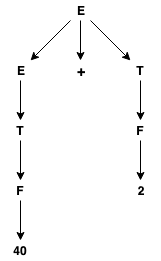
\includegraphics[keepaspectratio=true,scale=1]{figuras/parsetree.png}
	\caption{Exemplo de Parse Tree \cite{aho2006}.}
	\label{fig:parsetree}
\end{figure}

Um exemplo de \textit{parse tree} pode ser visto na Figura \ref{fig:parsetree}. Essa árvore significa a derivação
a seguir:

\begin{center}
    E => E + E => id + E => id + E * E => id + id * E => id + id * id
\end{center}

Segundo \cite{aho2006}, existem três tipos genéricos de \textit{parsers} para gramáticas 
livre de contexto: universal, \textit{top-down} e \textit{bottom-up}. Os métodos de \textit{parsing}
universais podem analisar qualquer gramática. Porém, são ineficientes.

Normalmente os métodos mais utilizados são  \textit{top-down} ou \textit{bottom-up}. Onde no primeiro
a \textit{parse tree} é construída a partir do topo, da raiz até as folhas. E no segundo é o inverso,
das folhas até a raiz. 

Vale ressaltar que os analisadores mais eficientes tanto \textit{top-down} ou \textit{bottom-up}  
só funcionam para subclasses de gramáticas livres do contexto. Este documento foca nos analisadores
do tipo \textit{top-down}.

\subsection{Analisadores \textit{Top-Down}}

Segundo \cite{aho2006}, a construção de analisadores do tipo \textit{top-down} é como o processo de
de construir a \textit{parse tree} a partir do topo e isto é
equivalente a encontrar a derivação mais à esquerda para a entrada.

\begin{lstlisting}[caption=Exemplo de gramática para analisadores top-down,label={lst:grammartopdown}]
E  ::= TE'

E' ::= '+'TE' | ''

T  ::= FT'

T' ::= '*'FT' | ''

F  ::= '('E')' | 'id'
\end{lstlisting}

Por exemplo dado a gramática descrita no Código \ref{lst:grammartopdown}, a análise sintática a partir do topo
consiste em cada etapa determinar qual produção aplicar para o não terminal. Depois que uma produção for escolhida
o processo resume-se a combinar os terminais no corpo da produção com os tokens da entrada. 

\begin{figure}[h]
	\centering
	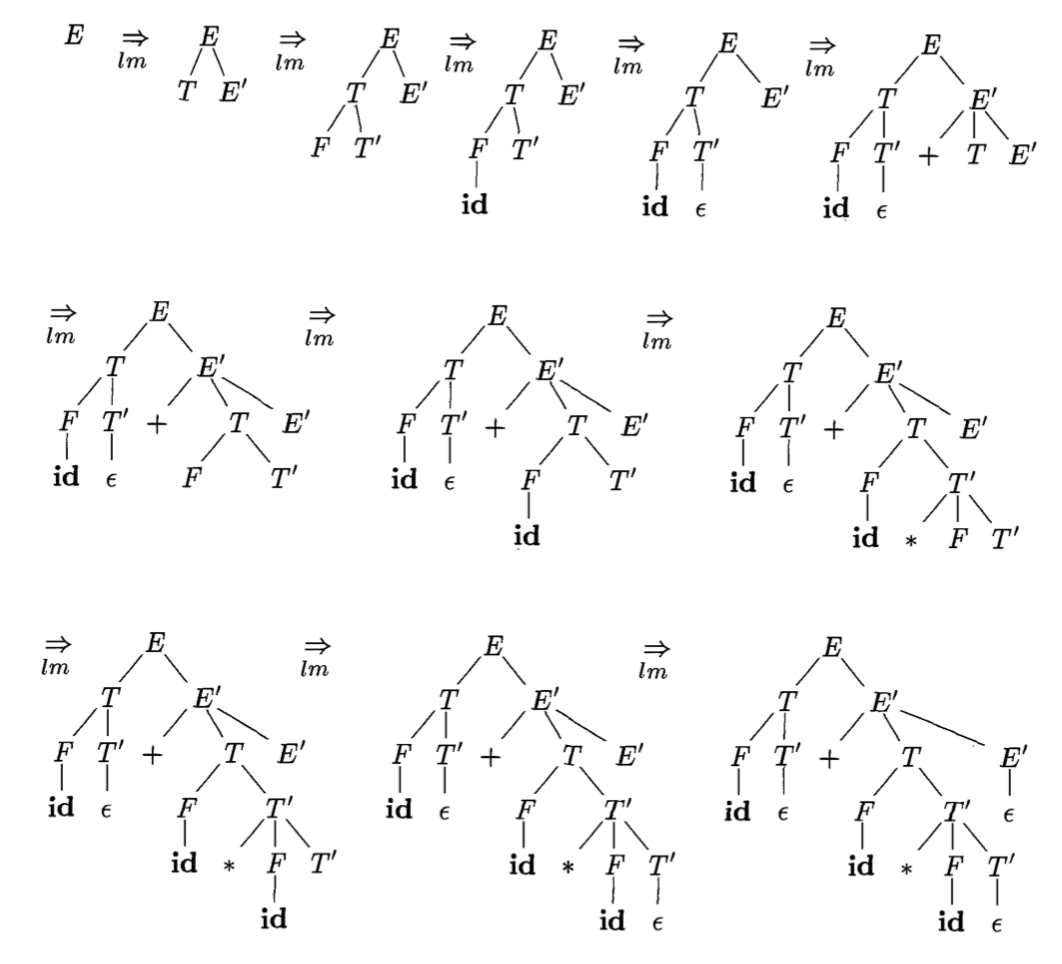
\includegraphics[keepaspectratio=true,scale=0.7]{figuras/parsetopdowntree.png}
	\caption{Exemplo de parse top-down \cite{aho2006}.}
	\label{fig:parsetopdowntree}
\end{figure}

Um exemplo de análise \textit{top-down} está na Figura \ref{fig:parsetopdowntree} 
onde existem várias árvores representando as derivações para a entrada \textbf{id + id * id}.

Descida recursiva é uma maneira simples e genérica para construir um \textit{parser top-down}.
Nesse tipo de analisador existe um conjunto de procedimentos para cada não terminal \cite{aho2006}. 

A execução começa chamando o procedimento para o símbolo inicial e então 
termina a execução com sucesso se a execução ler toda a entrada \cite{aho2006}. 

Esse tipo de analisador pode necessitar de \textit{backtracking}. Isto é, ler a entrada toda
novamente repetidas vezes. Pois caso o caminho tomado durante o momento de escolher uma produção falhar.
É necessário reiniciar a execução usando outra produção. A necessidade de recomeçar a execução
pode elevar o tempo de execução para valores exponenciais \cite{aho2006}. 

\begin{lstlisting}[caption=Exemplo de procedimento para um não terminal em descida recursiva,label={lst:recursive}]
def A():
    choose_A_production()
    for x in body_production:
        if is_nonterminal(x):
            procedure_for_x()
        elif x == current_token():
            next_token()
        else:
            error()
\end{lstlisting}

Um exemplo de procedimento para um não terminal pode ser visto no Código \ref{lst:recursive}.

Segundo \citeonline{aho2006}, para evitar a necessidade de \textit{backtracking}. 
Existe uma classe de parsers chamada preditiva. Ela consegue determinar a próxima produção 
a ser executada analisando os próximos tokens da entrada.

Esse tipo de analisador sintático pode ser construído para uma classe de gramática chamada LL(1), isto significa
ler a entrada da esquerda para a direita, encontrar a derivação mais à esquerda durante a execução e olhar 
apenas o token atual da entrada.

Para construir esse tipo de \textit{parser} é necessário uma abstração que permita escolher qual produção
a ser executada de maneira determinística.

Isto pode ser alcançado com uma \textit{predictive parsing table}. Essa tabela consiste
de linhas representando não terminais, colunas representando símbolo de entrada e o valor
dentro da célula diz qual produção escolher dado um não terminal e um símbolo.

O método para construir essa tabela necessita antes de duas operações comumente chamadas \textit{FIRST} e 
\textit{FOLLOW}.

A definição de FIRST(A), onde A é qualquer sequência de símbolos da gramática e portanto pode 
ser tanto terminal como não terminal, é o conjunto dos terminais que iniciam as 
sequências derivadas a partir de A. 

Como exemplo temos que, dado uma derivação A => ... => cy onde c é um terminal, 
logo c pertence ao conjunto FIRST(A). Pois inicia a sequência que foi derivada de A, isto é cy, 
e c é um terminal.

A definição de FOLLOW(A), onde A é um não terminal, é o conjunto de terminais x que podem aparecer imediatamente
a direita de A. Isto é, o conjunto de terminais x em derivações na forma S => ... => wAxy.

Com esses dois conjuntos pode-se construir a tabela preditiva. Com o seguinte algoritmo:

Para cada produção A ::= y da gramática.

\begin{itemize}
    \item Para cada terminal em FIRST(A), adicionar a produção A ::= y na tabela na linha do não terminal A e na coluna
    referente ao terminal.
    \item Se o terminal que representa caractere vazio estiver presente em FIRST(y). Então 
    adicionar a produção A ::= y na tabela. Especificamente na linha do não terminal A e 
    na coluna referente a cada terminal presente em FOLLOW(A).
\end{itemize}

Um exemplo de tabela preditiva pode ser visto em \ref{tbl:predictive}.

\begin{table}[h]
    \centering
	\caption{Tabela preditiva para analisador sintático LL(1)}
	\label{tbl:predictive}

    \begin{tabular}{cccccc}
        \toprule
        \multicolumn{1}{c}{\textbf{Não Terminal}} & \multicolumn{5}{c}{\textbf{Terminais}} \\
        \midrule
                       & \textbf{id} & \textbf{+} & \textbf{*} & \textbf{(} & \textbf{)}   \\
        \midrule
        \textbf{E}     & E ::= TE'  &            &             & E ::= TE'  &     \\
        \textbf{E}     &            & E' ::= +TE'&             &            & E ::= e   \\
        \textbf{T}     & T ::= FT'  &            &             & T ::= FT'  &     \\
        \textbf{T'}    &            & T' ::= e   & T' ::= *FT' &            & T' ::= e    \\
        \textbf{F}     & F ::= id   &            &             & F ::= (E)  &     \\
        \bottomrule
    \end{tabular}
\end{table}

Outro método para construir \textit{parsers top-down} bastante comum 
principalmente em linguagens funcionais são os chamados \textit{parsers combinators},
nesse modelo é construído um analisador com descida recursiva \cite{hutton1996monadic}.

Essa técnica utiliza funções como \textit{parsers} e define outras funções de alta ordem que
implementam abstrações das gramáticas livres de contexto, 
isto é, sequências, escolha e repetição \cite{hutton1996monadic}.

O método consiste em criar pequenos \textit{parsers} para as produções da gramática como funções. 
E utilzar as funções que representam as abstrações das gramáticas livres de contexto 
para combinar esses parsers \cite{hutton1996monadic}.

\section{Formatos para serialização de dados}

Nas seções anteriores foram discutidas maneiras para transformar um texto 
em uma representação computacional. Para tal foram definidas algumas abstrações
como linguagens, gramáticas e \textit{parsers}.

Como dito no Cap. \ref{sec:objective} o objetivo deste trabalho é definir
uma representação para troca de dados. Portanto é essencial discutir outras
notações existentes. Especialmente JSON (JavaScript Object Notation) e 
XML (Extensible Markup Language).

Segundo \citeonline{ecma404}, JSON é uma notação em formato de texto criada para facilitar 
a troca de dados entre sistemas. Foi baseada na linguagem JavaScript (ECMAScript). 
Tem o objetivo de ser fácil de ler e escrever e também ser fácil para máquinas interpretar e gerar.

Um valor JSON pode ser do tipo \textit{object}, \textit{array}, \textit{number}, \textit{string}, 
\textit{true}, \textit{false} ou \textit{null}. 

O tipo object é um conjunto de zero ou mais pares nome/valor. Um exemplo está em \ref{lst:jsonobj}

\begin{lstlisting}[caption=Exemplo de JSON Object,label={lst:jsonobj}]
    {
        "name" : "value",
        "name1" : 123
    }
\end{lstlisting}

Já o tipo array é um conjunto de valores JSON separados por virgúlas, como visto no exemplo \ref{lst:jsonarr}.

\begin{lstlisting}[caption=Exemplo de JSON Array,label={lst:jsonarr}]
    [123, "str", true, false, null]
\end{lstlisting}

A especificação do JSON propositalmente é simples. O objetivo é definir apenas a sintaxe e não a semântica
sobre como um valor JSON pode ser convertido para uma estrutura de dado de uma linguagem de programação.
A troca de dados entre sistemas usando JSON necessita de um acordo entre as partes envolvidas.

Outro formato muito conhecido é XML (Extensible Markup Language). Essa notação define os chamados documentos XML.
E também define parcialmente o comportamento dos processadores de XML \cite{XML}. 

Segundo \citeonline{XML}, para os documentos XML serem válidos eles devem seguir uma especificação, 
logicamente a abstração principal é o chamado elemento e um documento contém um ou mais elementos. 
Um elemento consiste de \textit{start-tags} e \textit{end-tags} ou no caso de um elemento vazio 
consiste de um \textit{empty-element tag}. Esses elementos possuem um tipo definido pelo seu nome e 
podem ter atributos. Como pode ser visto no exemplo \ref{lst:xmlelement}.

\begin{lstlisting}[caption=Exemplo de elementos XML,label={lst:xmlelement}]
    <termdef id="dt-dog" term="dog">duke</termdef>
    <foo>bar</foo>
    <br />
\end{lstlisting}

Existem também outros formatos tanto de texto como binários com foco na troca de dados
ou em representar arquivos de configuração. Para este trabalho os formatos \textit{Amazon Ion, edn e TOML}
trazem conceitos que evoluem os modelos JSON e XML.

\begin{itemize}
    \item \textbf{Amazon Ion}: Esta notação permite tanto texto como binário, o formato de texto
    é compátivel com JSON porém possui um modelo de dados com mais tipos, por exemplo blobs binários e
    timestamp.
    \item \textbf{TOML}: O formato TOML tem um foco em arquivos de configuração e em ser simples, 
    entretanto o modelo de dados também é mais diverso que o do JSON com tipos para datas por exemplo.
    \item \textbf{edn}: Este formato possui um modelo de dados rico e suporta um 
    mecanismo de extensibilidade para indicar mais semântica aos dados, esta abstração possui 
    alguma semelhança com o XML. Também suporta \textit{streaming} facilmente diferente de JSON.
\end{itemize}